\documentclass{article}

%-----------------------------------------------PACKAGES-------------------------------------------------------------%
\usepackage{graphicx} %images
\DeclareGraphicsExtensions{.pdf,.png,.jpg} % configures latex to look for the following image extensions
\usepackage{setspace} % allows for configuring the linespacing in the document
\usepackage{caption}
\usepackage{natbib}
\usepackage[a4paper, total={6in, 8in}]{geometry}
\usepackage[explicit]{titlesec}
\usepackage[toc,page]{appendix}
\usepackage{hyperref}
\usepackage[dvipsnames]{xcolor}
\usepackage{cleveref}
\setcounter{tocdepth}{2}
\usepackage[nottoc]{tocbibind}
\usepackage[parfill]{parskip}

\usepackage{listings} % to use code snippets 
\usepackage{color}

\usepackage{glossaries} % for glossary
\usepackage[final]{pdfpages}
\makeglossaries 
\newglossaryentry{API}
{
    name={API},
    text={API},
    description={Application programming interface. A set of endpoints which lead to functions and application logic. Allows developers to expose application functionality without directly exposing the code within the application}
}
\newglossaryentry{CRUD}
{
    name={CRUD},
    text={CRUD},
    description={Create, Read, Update, Delete. CRUD defines the four cornerstones of API functionality. An API should provide these functions to any user using the API}
}
\newglossaryentry{container}
{
    name={Container},
    text={container},
    description={An isolated piece of software bundled with everything it needs to run on the host}
}
\newglossaryentry{docker}
{
		name={Docker},
    text={Docker},
		description={A piece of software which enables orchestration and management of containers on a host}
}
\newglossaryentry{docker image}
{
		name={Docker Image},
		description={A template from which many containers can be started. Can be pushed an pulled to/from a remote Docker registry}
}
\newglossaryentry{docker daemon}
{
		name={Docker Daemon},
		description={The server-side component of the Docker Engine}
}
\newglossaryentry{lifecycle management}
{
		name={Lifecycle Management},
    text={lifecycle management},
		description={The management of a container over its complete lifecycle, from its beginnings as an image to starting, stopping and restarting the container and managing the interactions it has with other containers on the system}
}
\newglossaryentry{continuous integration}
{
		name={Continuos Integration},
		description={The act of continuously merging newly created software with the current working version, validated by automatic build and testing tools allowing for early detection of faults}
}
\newglossaryentry{continuos deployment}
{
		name={Continuos Deployment},
		description={The act of continuously deploying software which has passed acceptance tests to a live system}
}
\newglossaryentry{command line}
{
    name={Command Line},
    text={command line},
    description={The program through which the operating system can be interacted with. The user enters a command they wish to execute on a text line}
}
\newglossaryentry{open source}
{
    name={Open Source},
    text={open source},
    description={Software which encourages input and feedback from other developers and allows for any and all modifications to the current software package with the intent to release it under a new package}
}
\newglossaryentry{technical debt}
{
    name={Technical Debt},
    text={technical debt},
    description={The extra development work which arises as a result of implementing an easier but less robust solution}
}
\newglossaryentry{sonarqube}
{
    name={SonarQube},
    text={SonarQube},
    description={A tool to scan source code. It can inform developers of coding best-practices and highlight ``code smells'', which are essentially when best practices are not adhered to. Also highlights technical debt. Code is deemed either `passing' or `failing', meaning the code has been deemed either sufficient or insufficient in the following categories: Code Test Coverage, Bugs, Vulnerabilities and Technical Debt Ratio}
}
\newglossaryentry{travis}
{
    name={Travis},
    text={Travis},
    description={A website which allows for automatic builds of code and feedback of results. Can be used to automatically deploy code dependent on test results also}
}
\newglossaryentry{git}
{
    name={Git},
    description={A version control system which allows source code to be tightly controlled and stored in a central repository}
}
\newglossaryentry{github}
{
    name={Github},
    text={Github},
    description={An online platform to store git repositories. Allows for multi-developer collaboration on projects}
}
\newglossaryentry{Docker Compose}
{
    name={Docker Compose},
    description={A tool developed by Docker to allow developers to easily orchestrate multi-container systems without requiring them to manually manage containers}
}
 

\definecolor{lightgray}{rgb}{.9,.9,.9}
\definecolor{darkgray}{rgb}{.4,.4,.4}
\definecolor{purple}{rgb}{0.65, 0.12, 0.82}

\lstdefinelanguage{JavaScript}{
  keywords={typeof, new, true, false, catch, function, return, null, catch, switch, var, if, const, let, in, while, do, else, case, break, require},
  keywordstyle=\color{blue}\bfseries,
  ndkeywords={class, export, exports, boolean, throw, implements, import, this},
  ndkeywordstyle=\color{darkgray}\bfseries,
  identifierstyle=\color{black},
  sensitive=false,
  comment=[l]{//},
  morecomment=[s]{/*}{*/},
  commentstyle=\color{purple}\ttfamily,
  stringstyle=\color{red}\ttfamily,
  morestring=[b]',
  morestring=[b]"
}

\lstset{
   language=JavaScript,
   backgroundcolor=\color{lightgray},
   extendedchars=true,
   basicstyle=\footnotesize\ttfamily,
   showstringspaces=false,
   showspaces=false,
   numbers=left,
   numberstyle=\footnotesize,
   numbersep=9pt,
   tabsize=2,
   breaklines=true,
   showtabs=false,
   captionpos=b
}
\usepackage{hyperref}
\newcommand\myshade{85}
\colorlet{mylinkcolor}{NavyBlue}
\colorlet{mycitecolor}{YellowOrange}
\colorlet{myurlcolor}{Aquamarine}

\hypersetup{
  linkcolor  = mylinkcolor!\myshade!black,
  linktocpage=true,
  citecolor  = mycitecolor!\myshade!black,
  urlcolor   = myurlcolor!\myshade!black,
  colorlinks = true,
}

\bibliographystyle{agsm}
\setcitestyle{authoryear,open={(},close={)}}

\begin{document}
\onehalfspacing
\hypersetup{pageanchor=false}
% !TEX root = ../final_report.tex
\begin{titlepage}
	\centering
	\mbox{}\\
	\mbox{}\\
	\mbox{}\\
	{\huge\bfseries Lifecycle Management for Docker UI \par}
	{\Large\bfseries \textit{Gantry}\par}
	\vspace{1cm}
	{\scshape\large Final Report (Semester 2)\par}
	\vspace{3cm}
	{\Large Stephen Coady\par}
	{\Large 20064122\par}
	\vspace{3cm}\par
	\vfill
	{\Large Dr.~Brenda \textsc{Mullally}}
	\vspace{1cm}\par
	{\Large BSc (Hons) in Applied Computing\par}

  % {\large \today\par}

	\vfill
	
	\clearpage
	\thispagestyle{empty}
	\centering
	\mbox{}\\
	\mbox{}\\
	\begin{figure}[!ht]
	\centering
	\includegraphics*[width=0.7\textwidth]{images/gantry-single-darktext}
	\label{fig:gantry-single-darktext}
	\end{figure}
	
	{\huge\bfseries Gantry: Lifecycle Management For Docker UI \par}
	\vspace{1cm}
	{\Large \textit{Stephen Coady}\par}
	\vspace{3cm}\par
	\vfill
	\vspace{1cm}\par

	% {\large \today\par}

	\vfill
% Bottom of the page
\end{titlepage}

\hypersetup{pageanchor=true}
\clearpage
\begin{center}
\begin{minipage}{\textwidth}
  
  {\scshape\large \textbf{Plagiarism Declaration}\par}
  \vspace{1cm}
  Unless otherwise stated all the work contained in this report is my own.  I also state that I have not submitted this work for any other course of study leading to an academic award.
\end{minipage}
\end{center}
\vfill % equivalent to \vspace{\fill}
\clearpage

\tableofcontents

\newpage
\printglossaries

\newpage
% !TEX root = ../report_v2.tex
\section{Introduction}
\label{sec:intro}
This report will aim to guide the reader through the planning and development of the Lifecycle Management for Docker \gls{UI} application. After reading this report the reader should have a clear idea of why the application was built, what was used to build it and how the process was carried out.

This application will be built using open source principles and best practices, enabling it to be maintained and improved by any developer who wishes to contribute. For this reason many of the decisions made and processes employed were done so with an open source final product in mind.

\subsection{Problem Statement}
Currently the \gls{Docker} application does not ship with any bundled \gls{UI}. When installed, it is comprised of a client and a server side component \citep{Docker2017}. The server side exposes itself through an \gls{API} and is ultimately responsible for controlling all aspects of Docker on the host such as containers, images, networks and volumes etc. The API exposed by the server-side application of the Docker Engine is consumed by the Docker \gls{CLI} which is the client side application. A graphical representation of the complete Docker engine can be seen in Figure \ref{fig:docker_engine}.

\begin{figure}[!ht]
\centering
\includegraphics*[width=0.7\textwidth]{images/docker_engine}
\caption{\em Docker Engine Components. Credit: \citep{Docker2017}}
\label{fig:docker_engine}
\end{figure}

This model is extremely versatile as it allows the developer to control any \gls{Docker daemon} (the server-side component of a Docker installation) once they have access to the command line of the host Docker is running on. In fact, if the API exposed by the Docker daemon is exposed remotely then the developer does not need access to the host's command line, instead they can directly access the API remotely.

While the \gls{CLI} gives developers full control over the server-side component of a \gls{Docker host} it also has its drawbacks.

\begin{itemize}
	\item Learning curve - the person using the command line must be familiar with typical commands used to achieve certain tasks. This precludes anybody without these skills from using Docker.
	\item Vast set of Docker commands - there are a vast number of commands available to use from the Docker CLI. This is also a learning curve as even a developer who is familiar with a CLI must first learn the Docker commands to be able to use the client-side application. 
	\item User friendliness - The command line does not produce content that is easily readable and can often format the data it is trying to present in an odd fashion depending on things like screen size etc.
\end{itemize}

\subsection{Aims and Objectives}
\label{sub:aims}
The aim of this project is to address all of these problems while also trying to increase the functionality available to anybody who wishes to use Docker.

At a high level the primary objectives of this project are:

\begin{itemize}
	\item Fully functional server-side application
	\item Expose this application through a \gls{REST}ful API.
	\item A fully functional front-end application
	\item A \gls{Docker image} built to allow easy distribution of the application
\end{itemize}

These objectives will then provide the following functionality:

\begin{itemize}
	\item A UI which will 
	\begin{itemize}
		\item allow users to manipulate images, containers etc on the host with the same capabilities as the command line
		\item allow them to do this remotely
	\end{itemize}
	\item A runnable container which has no other dependencies so that it can be run without installing the application
	\item An independent API which can be consumed by any front end application
	\begin{itemize}
		\item This will provide flexibility if the front end framework needs to be changed further down the line
	\end{itemize}
\end{itemize}


\newpage
\section{Technologies}
In this section of the report the technologies used to create the application will be examined and explained in detail.
\subsection{Docker}
\gls{Docker} is a platform which allows developers to package their applications into isolated containers which contain only the software dependencies required by the application. A container is different to a \gls{VM} in that a container does not contain a full operating system \citep{WhatDocker}.

Since a primary objective of this application is to manage a \gls{Docker host} it makes sense to leverage the capabilities of Docker and run this application within a \gls{Docker container}. This provides several benefits over distributing source code, such as:

\begin{itemize}
	\item Portability - If a \gls{Docker image} can be built and uploaded to a public repository then it makes it easier for other developers to pull and run the application.
	\item Ease of use - As the application will be running in a container a developer does not need to install any third party components on their system to use the application. They do not need to worry about their environment at all, once their system has Docker installed it will run the application.
	\item Ephemeral - Docker containers are designed to be `throw-away'. This means that if this application needs to be quickly stopped and restarted then containers are the perfect vehicle to do this.
\end{itemize}
\subsection{Node JS}
\label{sub:nodejs}
Node JS is a server-side JavaScript runtime, it is built on the same V8 engine that powers the popular Chrome browser. It uses an event-driven, non-blocking I/O model that makes it lightweight, efficient and very fast. Node JS' package ecosystem, NPM, is the largest ecosystem of open source libraries in the world. \citep{Nodejs.org2016}. Node JS provides an excellent way to build highly scalable network application which are non blocking and extremely performant \citep{Griffin2011}. This means that if the application was adapted in the future to deal with large numbers of servers then the technology choice will be able to deal with that.

Node JS was also deemed a good fit for this project as it has a large and extremely active online community. Since this is an open source project this will increase the likelihood of other developers taking part in the project and contributing. We can see in Figure \ref{fig:counts} that there are currently (as of November 2016) more node modules available through the node package manager (NPM) than any other of the large package managers such as the ones used by Go, PHP, Python and Ruby. 

\begin{figure}[!ht]
\centering
\includegraphics*[width=0.7\textwidth]{images/module_counts}
\caption{\em Various Module Counts (Credit: modulecounts.com)}
\label{fig:counts}
\end{figure}

\subsection{Angular JS}
Angular JS is a web framework for building dynamic web applications using Javascript as a controller. It uses HTML as its template language to display the information passed to it from the application controller \citep{Angular2017}. 

For this application the front end requirements were relatively low. Once the framework provided a mechanism to show dynamic content then it was a candidate. For this reason several were evaluated and Angular was chosen as it had the lowest barrier to entry. The front-end application will be discussed further in Section \ref{sec:design}.

\subsection{Travis CI}
Since this project was developed as an open source project it made sense to have a transparent and fully automated build process integrated into the project. For this reason \gls{continuous integration} in this project is handled by \gls{Travis} CI. It is a feature-rich service free to use for open source projects and has a large user base. The set up used in this project for testing and continuous integration will be explored further in Section \ref{sec:methodology}.

\subsection{Vagrant}
Vagrant is a technology to create configurable, reproducible and portable environments by using a set of programmable steps to produce a \gls{VM} which the developer can use to develop in \citep{Vagrant2017}. While this is just one use-case of Vagrant it is the main reason it was used in this project. 

Since this project is open source it is useful to have one standardised VM within which all development can take place. This virtual machine can then be shared (either as its own separate repository or included in the main application repository). This is useful as it enables any developer who wishes to contribute to the project to instantly have the required environment. For instance, a developer can contribute to this project by using the \gls{Vagrantfile} supplied without requiring them to first install Docker or Node JS.


\newpage
\section{Design and Implementation}

\subsection{Front End Application}

To show conceptually how the application may look a wireframe of the user-facing application was built. It will give the reader some indication of what the final application will look like. While it is only at conceptual level it does encapsulate the primary goals and how they will be implemented. It shows how images and containers can be listed and interacted with, allowing with performing advanced actions on them. This wireframe can be seen in Figure \ref{fig:wireframe}.
\begin{figure}[!ht]
\centering
\makebox[\textwidth]{\includegraphics*[width=0.7\paperwidth]{images/wireframe}}
\caption{\em Wireframe}
\label{fig:wireframe}
\end{figure}

\subsection{Class Diagram}
We can also see the conceptual class diagram for the system in Figure \ref{fig:class_diagram}. It should be noted that while all aspects of the Docker ecosystem are modelled in Figure \ref{fig:class_diagram} they are not all local objects. This is highlighted by distinguishing between the local and remote systems. It is still important to show the remote system's relationship with the local system as many local actions will be affected by the remote system.

\begin{figure}[!ht]
\centering
\makebox[\textwidth]{\includegraphics*[width=0.9\paperwidth]{images/docker_class_diagram}}
\caption{\em Class Diagram}
\label{fig:class_diagram}
\end{figure}

We can see in Figure \ref{fig:class_diagram} that from a data-modelling perspective the system is quite small, this is due to the nature of Docker and how most data will be stored and managed by Docker itself. Since the database being used will be NoSQL the concept of relationships does not strictly apply, however they are modelled for clarity.

\subsection{Sequence Diagram}

To obtain a clearer understanding of how basic create, read, update and delete functions will operate throughout the various levels of the application - we can use sequence diagrams. Figure \ref{fig:sequence_diagram} aims to show the sequence of events contained in these basic functions. Note that not all functions are modelled using sequence diagrams as they are too numerous to do, however the sequence of events for each are quite similar to that shown in Figure \ref{fig:sequence_diagram}.

\begin{figure}[!ht]
\centering
\makebox[\textwidth]{\includegraphics*[width=0.9\paperwidth]{images/docker_system}}
\caption{\em Sequence Diagram}
\label{fig:sequence_diagram}
\end{figure}

We can also use sequence diagrams to show the flow of the user login and registration aspect of the application since this is quite different to the Docker side. This aims to show the sequence of events when a user tries to register with the application and then when they try to log in. This can be seen in Figure \ref{fig:user_sequence_diagram}.

\begin{figure}[!ht]
\centering
\makebox[\textwidth]{\includegraphics*[width=0.8\paperwidth]{images/user_system}}
\caption{\em User System Sequence Diagram}
\label{fig:user_sequence_diagram}
\end{figure}

\subsection{Use Case Diagram}

Now that we have an understanding of the components of the system and how they interact with each other to perform specific functions we can now look at a use case diagram which aims to tie together the basic use cases of the system. We can see this in Figure \ref{fig:use_case_diagram}. As before, a subset of use cases which accurately encompass other uses of the system have been chosen here, as a larger use case diagram would not be beneficial to understanding the system better. 

\begin{figure}[!ht]
\centering
\makebox[\textwidth]{\includegraphics*[width=0.9\paperwidth]{images/use_case}}
\caption{\em Use Case Diagram}
\label{fig:use_case_diagram}
\end{figure}

\newpage
\subsection{Implementation}
To implement the system outlined in this section, some initial tickets were detailed. These were grouped under the Agile headings of:

\begin{itemize}
	\item Epics - which describe a large feature set of the system.
	\item Tickets - the sub group under which the tasks to get an epic completed can be placed
	\item Sub Tasks - which are the smallest units of work. When all sub tasks for a ticket is completed then that ticket is said to be completed.
\end{itemize}

To prioritise the tasks within this project each ticket was given two scores. The first was a priority score which gives an indication as to how vital this ticket is to the overall project. An indication of this can be seen in Section \ref{sub:goals}. The second score is an estimate of the complexity of completing said task. Together, these two scores are combined to give an overall weighting to each ticket, thereby making it easier to decide which tasks should be taken first. Tasks with a higher overall score are more likely to be worked on sooner. We will know look at the first draft of project epics and their respective tickets.

\newpage
\paragraph{Docker Image CRUD}\mbox{}\\
This section will look at the basic Docker Image tasks of the system. Completion of this epic will allow the user to have complete control over all Docker images on the system.

\begin{figure}[!htbp]
\centering
\makebox[\textwidth]{\includegraphics*[width=0.8\paperwidth]{images/images-crud}}
\end{figure}

\paragraph{Docker Container Management}\mbox{}\\
This section will deal with container management. When completed, a user should have total control over all containers, both running and otherwise on the system.

\begin{figure}[!htbp]
\centering
\makebox[\textwidth]{\includegraphics*[width=0.8\paperwidth]{images/container-crud}}
\end{figure}

\newpage
\paragraph{Security Epic}\mbox{}\\
Security of the system is also an epic. This will mean both how the system is accessed by a user, as certain users may be accessing the system remotely. It will also include how the access occurs, i.e. will the application use SSL certificates to encrypt data flow to and from the application.

\begin{figure}[!htbp]
\centering
\makebox[\textwidth]{\includegraphics*[width=0.8\paperwidth]{images/security}}
\end{figure}

\paragraph{Core Application Epic}\mbox{}\\
This section will look at some of the broader details of the project. 

\begin{figure}[!htbp]
\centering
\makebox[\textwidth]{\includegraphics*[width=0.8\paperwidth]{images/core-application}}
\end{figure}


\newpage
\section{Methodology}
\label{sec:methodology}
\subsection{Agile}
\subsection{Jira}
\subsection{Gitflow}
\subsection{Testing}
\subsection{Continuous Integration/Deployment}


\newpage
\appendix
\section*{Appendices}
\addcontentsline{toc}{section}{Appendices}
\renewcommand{\thesubsection}{\Alph{subsection}}

\subsection{Application Repository}
\label{appendix:code}
https://github.com/StephenCoady/lifecycle-management-for-docker

\subsection{Dockerode} 
\label{appendix:dockerode_appendix}
https://github.com/apocas/dockerode

\subsection{Travis Repository} 
\label{appendix:travis}
https://travis-ci.org/StephenCoady/lifecycle-management-for-docker

\subsection{SonarQube Repository} 
\label{appendix:sonarqube}
https://sonarqube.com/dashboard/index?id=lifecyle-management-for-docker

\subsection{Sprint Retrospectives}
\label{appendix:retros}
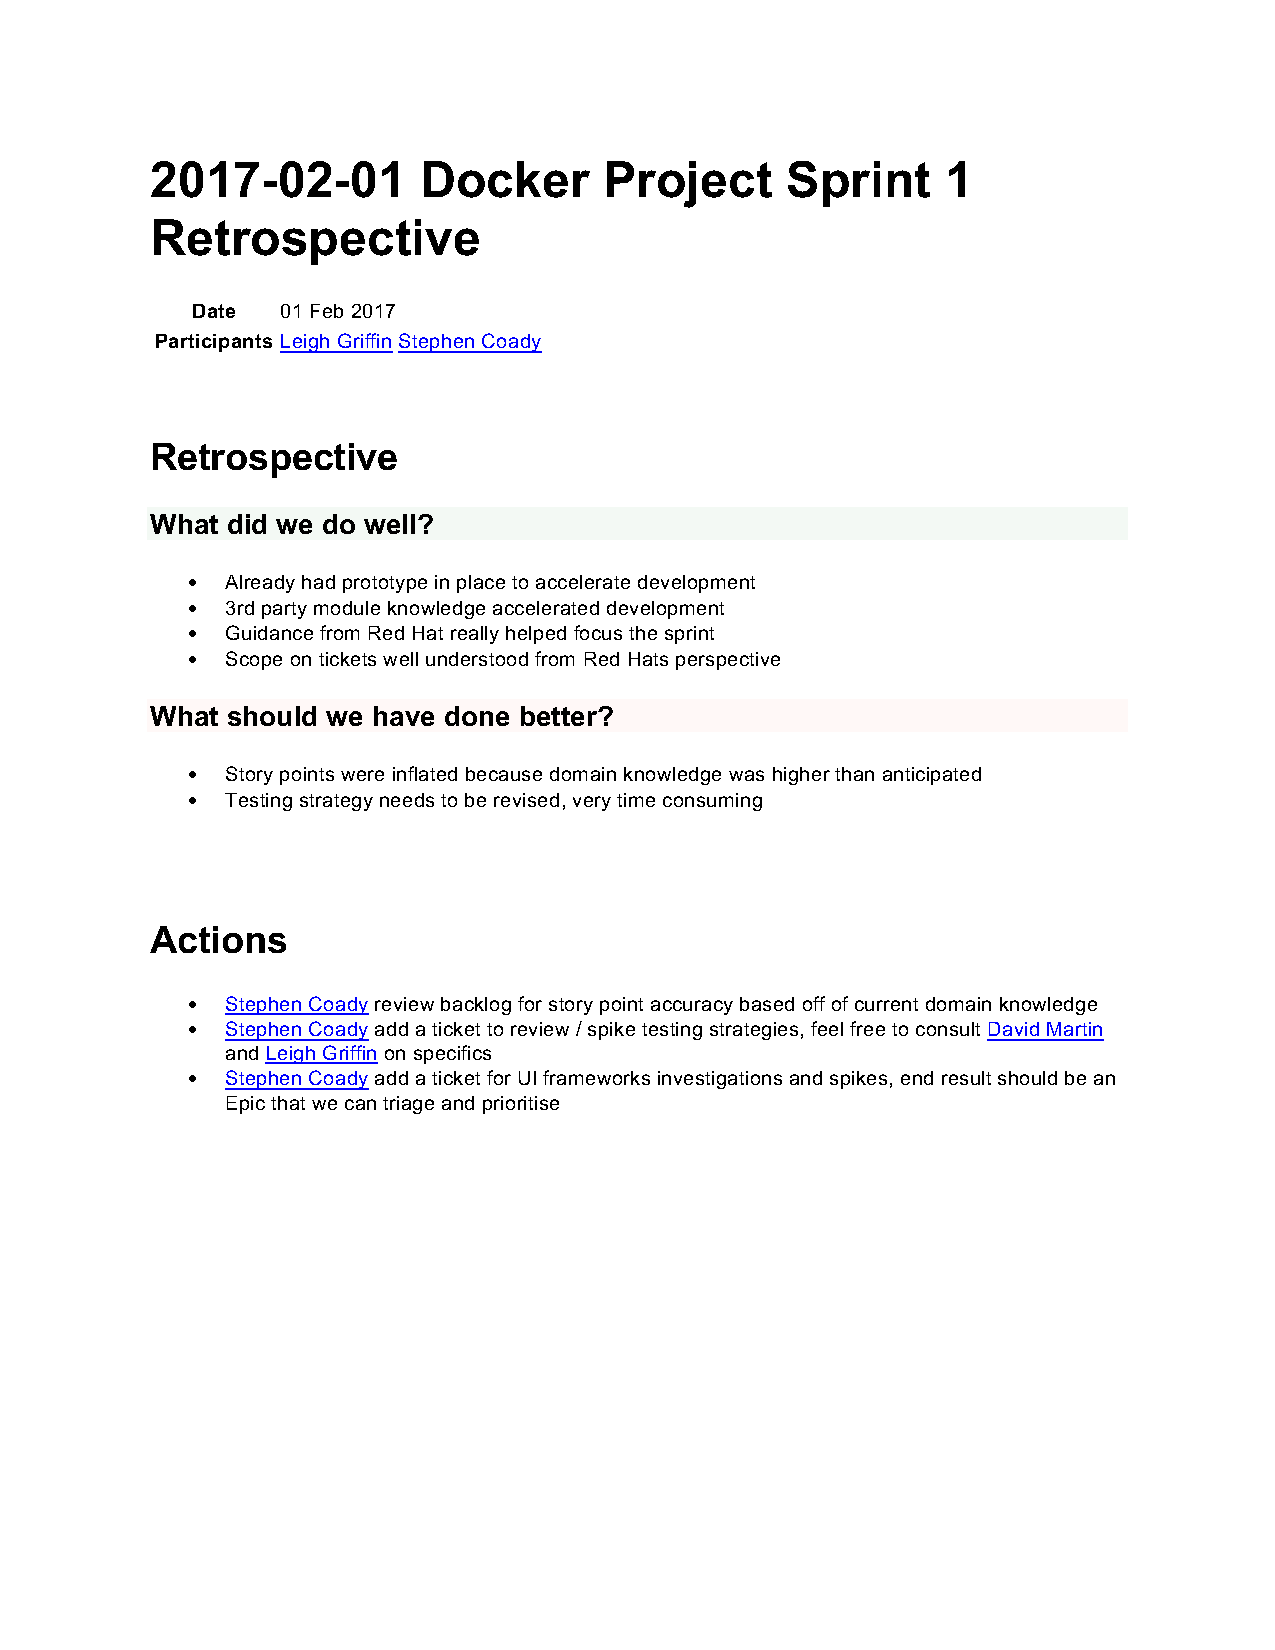
\includepdf[pages=-,pagecommand={}]{components/retrospectives/sprint_1_retrospective.pdf}
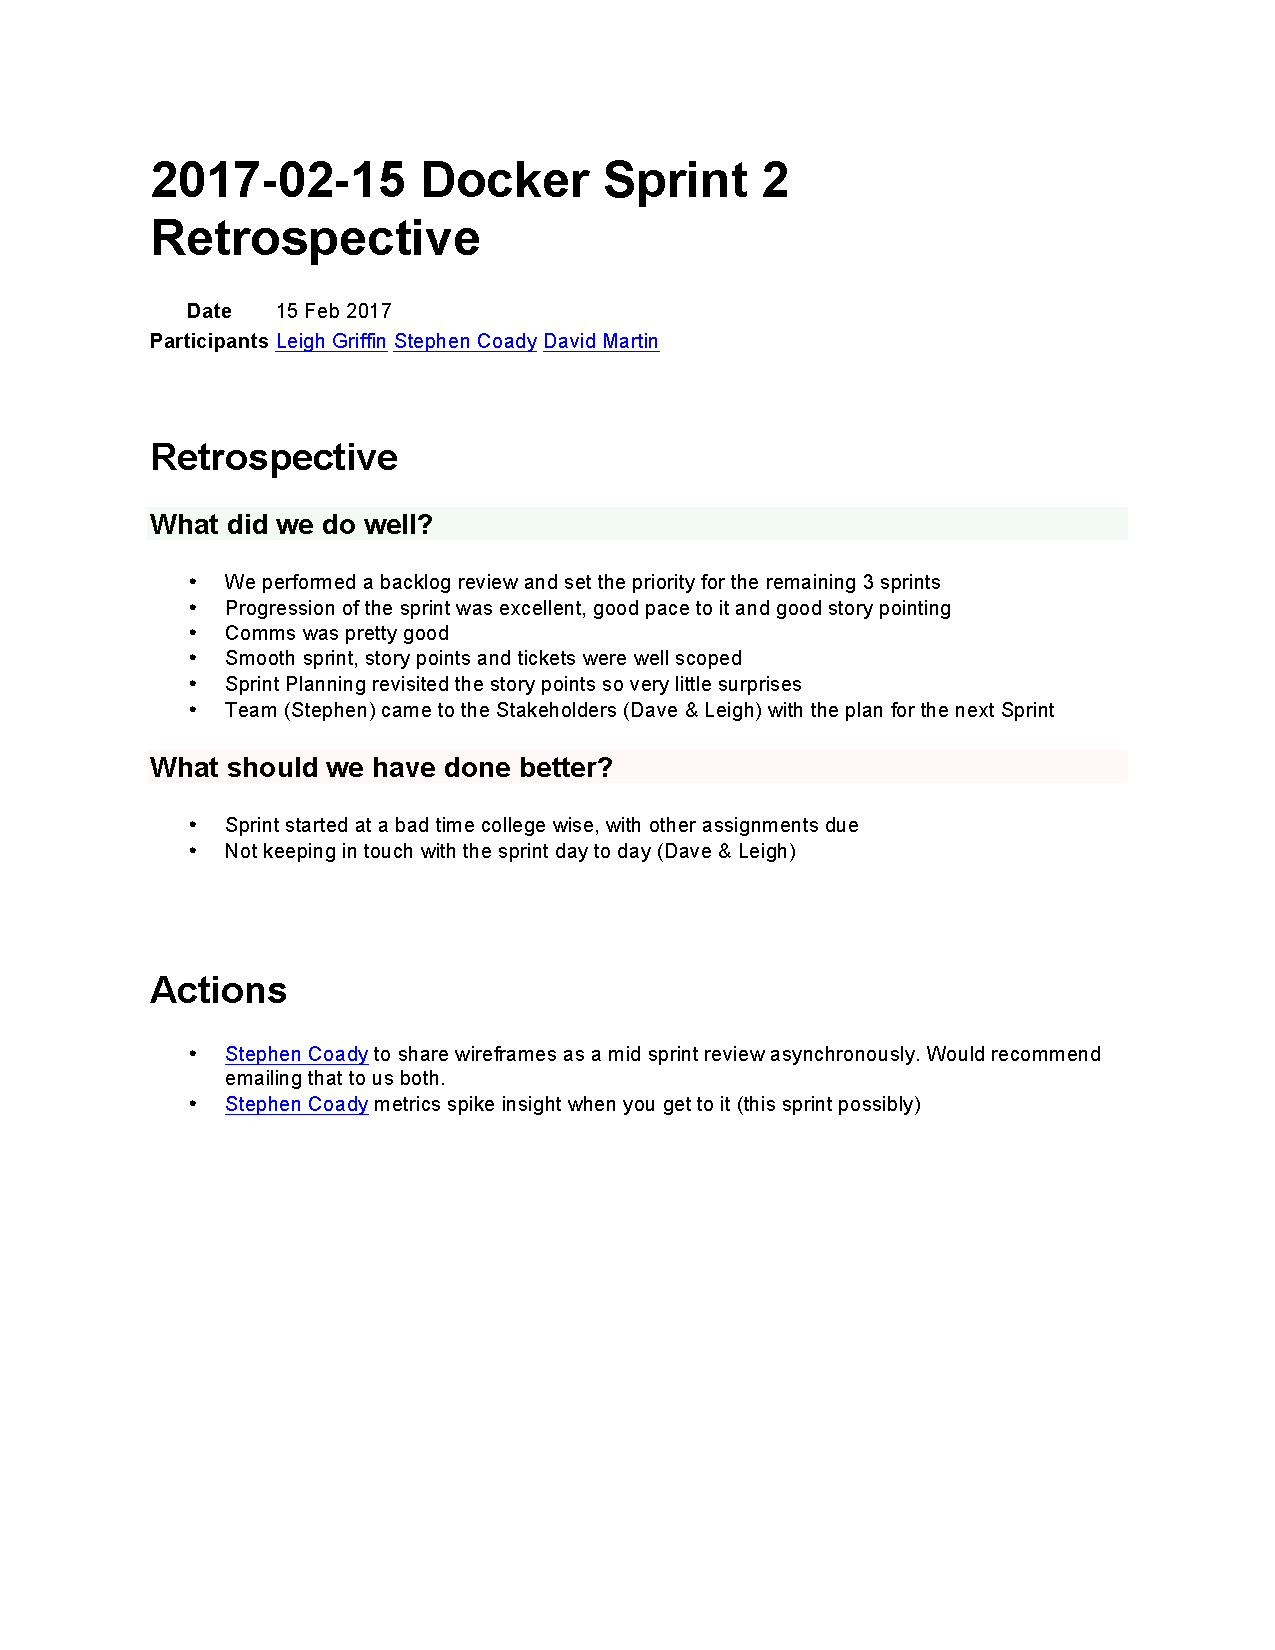
\includepdf[pages=-,pagecommand={}]{components/retrospectives/sprint_2_retrospective.pdf}
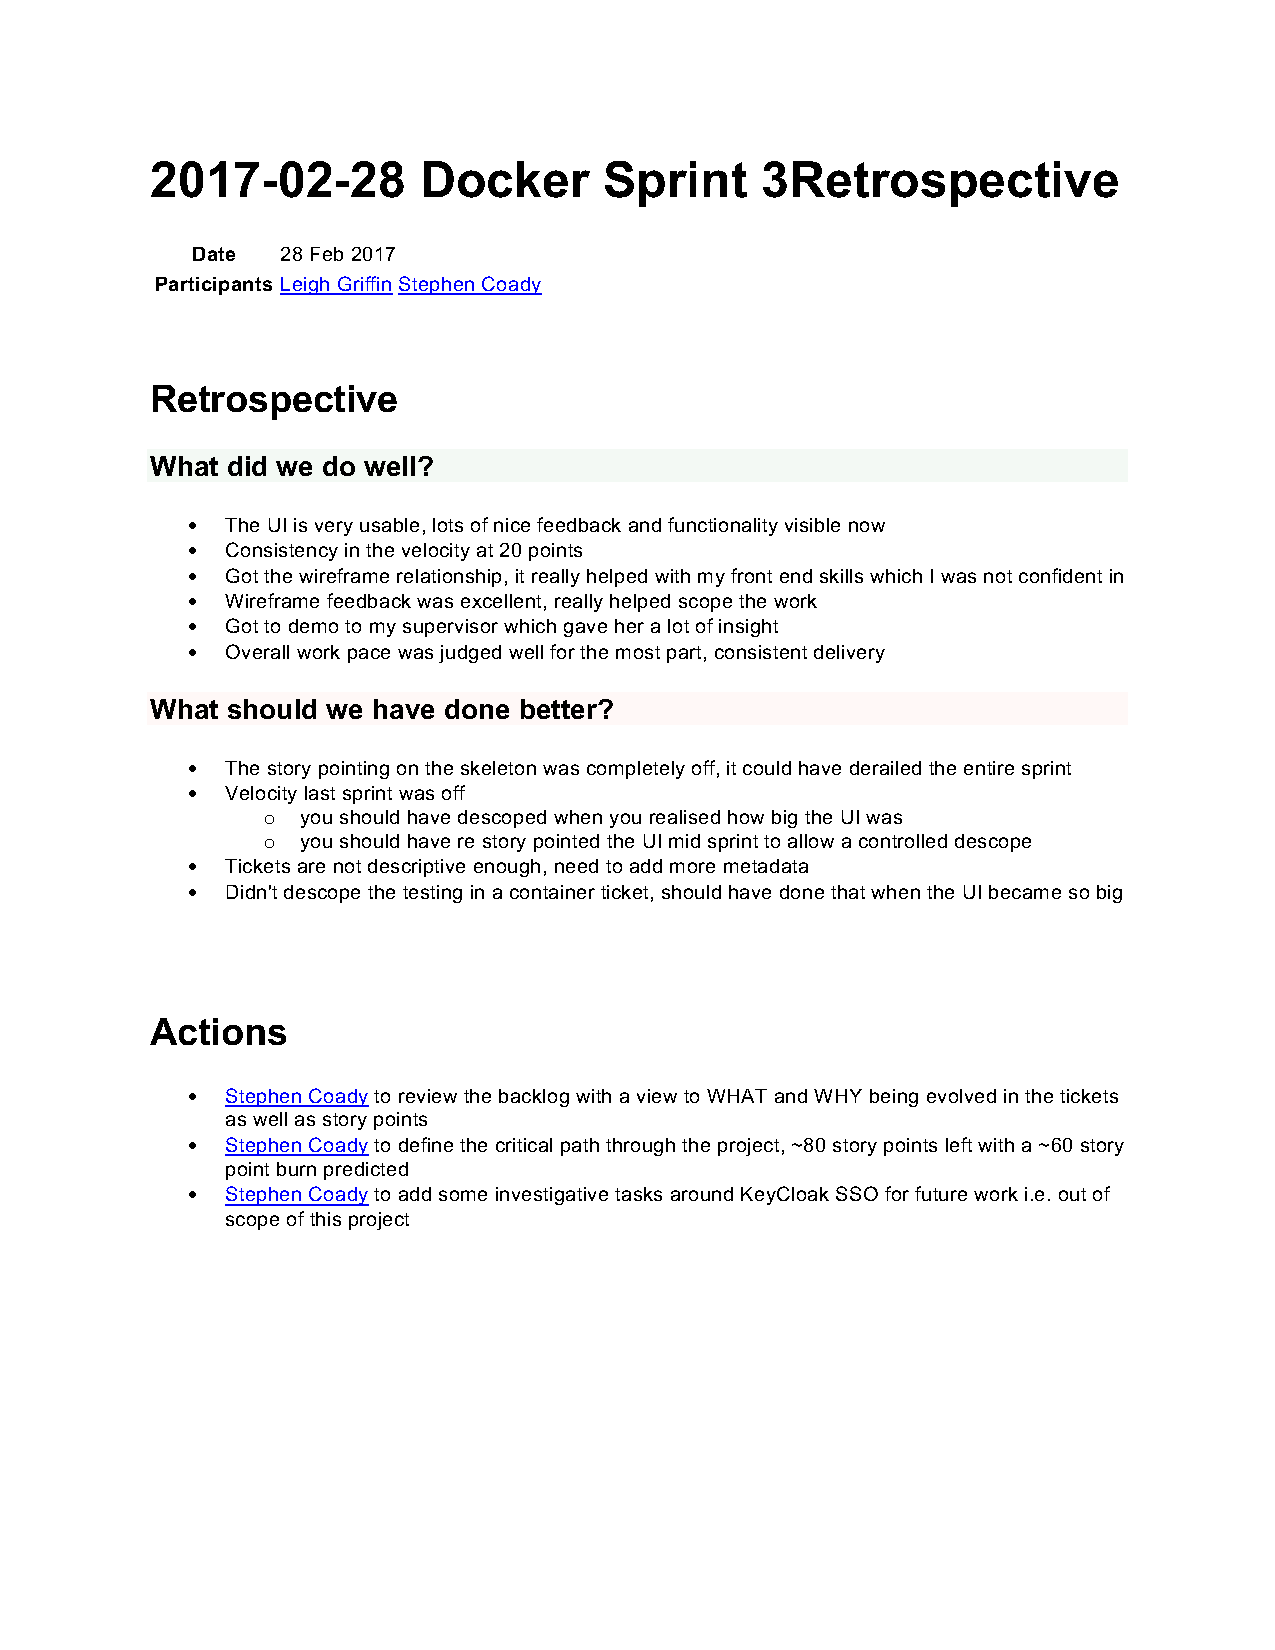
\includepdf[pages=-,pagecommand={}]{components/retrospectives/sprint_3_retrospective.pdf}


\newpage
\bibliography{bibliography}

\end{document}
